%%%%%%%%%%%%%%%%%%%%%%%%%%%%%%%%%%%%%%%%%%%%%%%%%%%%%%%%%%%%%%%%%%%%%%%%%%%%%%%%
%2345678901234567890123456789012345678901234567890123456789012345678901234567890
%        1         2         3         4         5         6         7         8

\documentclass[letterpaper, 10 pt, conference]{ieeeconf}  % Comment this line out
                                                          % if you need a4paper
%\documentclass[a4paper, 10pt, conference]{ieeeconf}      % Use this line for a4
                                        % paper
\usepackage{graphicx}
\usepackage{amssymb}
\usepackage{amsmath}
\usepackage{breqn}
\IEEEoverridecommandlockouts                              % This command is only
                                                          % needed if you want to
                                                          % use the \thanks command
\overrideIEEEmargins
% See the \addtolength command later in the file to balance the column lengths
% on the last page of the document



% The following packages can be found on http:\\www.ctan.org
%\usepackage{graphics} % for pdf, bitmapped graphics files
%\usepackage{epsfig} % for postscript graphics files
%\usepackage{mathptmx} % assumes new font selection scheme installed
%\usepackage{times} % assumes new font selection scheme installed
%\usepackage{amsmath} % assumes amsmath package installed
%\usepackage{amssymb}  % assumes amsmath package installed

\title{\LARGE \bf
An\'alisis de la condici\'on de guiamiento en gu\'ias de onda diel\'ectricos del tipo SLAB
}

%\author{ \parbox{3 in}{\centering Huibert Kwakernaak*
%         \thanks{*Use the $\backslash$thanks command to put information here}\\
%         Faculty of Electrical Engineering, Mathematics and Computer Science\\
%         University of Twente\\
%         7500 AE Enschede, The Netherlands\\
%         {\tt\small h.kwakernaak@autsubmit.com}}
%         \hspace*{ 0.5 in}
%         \parbox{3 in}{ \centering Pradeep Misra**
%         \thanks{**The footnote marks may be inserted manually}\\
%        Department of Electrical Engineering \\
%         Wright State University\\
%         Dayton, OH 45435, USA\\
%         {\tt\small pmisra@cs.wright.edu}}
%}

\author{Cesar J. Munoz Martinez$^{1}$% <-this % stops a space
\thanks{Este trabajo es realizado para la tarea 1 del curso de \'optica integrada}% <-this % stops a space
\thanks{$^{1}$Unidad de Postgrado de la Facultad de Ingenieria Electrica y electronica,
        Universidad Nacional de Ingenieria}%
}


\begin{document}



\maketitle
\thispagestyle{empty}
\pagestyle{empty}


%%%%%%%%%%%%%%%%%%%%%%%%%%%%%%%%%%%%%%%%%%%%%%%%%%%%%%%%%%%%%%%%%%%%%%%%%%%%%%%%
\begin{abstract}

Esta publicaci\'on discute los temas de la formaci\'on de ondas \'opticas dentro de gu\'ias de ondas SLAB, los cuales est\'an conformados por tres capas, cada una con diferente \'indice de refracci\'on. Se observa la formaci\'on ondas TE (Transversal El\'ectrico) y ondas TM (Transversal Magn\'etico) cuyo comportamiento es regido por las Ecuaciones de Maxwell y la distribuci\'on de los campos que lo conforman.

\end{abstract}


%%%%%%%%%%%%%%%%%%%%%%%%%%%%%%%%%%%%%%%%%%%%%%%%%%%%%%%%%%%%%%%%%%%%%%%%%%%%%%%%
\section{INTRODUCCI\'ON}

Se conoce como  gu\'ia de ondas a cualquier estructura f\'isica capaz de guiar ondas electromagn\'eticas, en el cual el medio diel\'etrico donde se transmite estas ondas electromagn\'eticas esta limitado por otro material diel\'ectrico (Ver Figura~\ref{fig:WaveGuideSlab1}). La transmisi\'on de la informaci\'on a trav\'es de gu\'ias de ondas es m\'as adecuada a frecuencias HF (Alta Frecuencia) debido a que se produce menor atenuaci\'on que en otros medios de transmisi\'on. En el proceso de an\'alisis de esta publicaci\'on se considera campos arm\'onicos en el tiempo, condiciones uniformes e isotr\'opicas y que el factor de propagaci\'on se encuentra presente en todos los componentes de los campos el\'ectrico y magn\'etico.

% +++Figura 1+++
\begin{figure}[ht!]
\centering{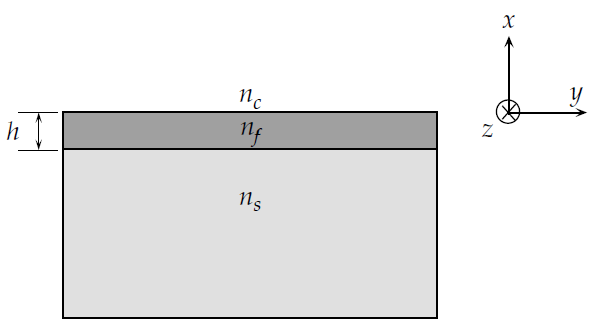
\includegraphics[width=80mm]{imagenes/WaveGuideSlab1.png}}
\caption{Modelos de gu\'ias de onda \'opticos de estructura bidimensional (a) y tridimensional (b) y (c). Fuente:
}\label{fig:WaveGuideSlab1}
\end{figure}

\section{DEDUCCI\'ON DEL COMPORTAMIENTO F\'ISICO}

\subsection{Derivaci\'on a partir de las ecuaciones de la ley del Eletromagnetismo}

Las ecuaciones~\eqref{eq:MaxwellEquation1}, ~\eqref{eq:MaxwellEquation2}, ~\eqref{eq:MaxwellEquation3} y ~\eqref{eq:MaxwellEquation4}, son las ecuaciones de Maxwell que rigen las leyes del electromagnetismo, para nuestro caso especial que trata el comportamiento de la onda en guias de onda dielictrica se hace las siguientes consideraciones: 
\begin{itemize}
  \item Inexistencia de Cargas el\'ectricas y magn\'eticas.
  \item Fuentes de Corriente el\'ectrica y densidad el\'ectrica nulas
  \item Material en condiciones constitutivas magn\'eticas, uniforme, lineal e isotr\'opico
  \item Medio f\'isico sin p\'erdidas
\end{itemize}
\begin{equation}
\label{eq:MaxwellEquation1}
{
\nabla  \times \vec E =  - {{\vec M}_i} - \frac{{\partial \vec B}}{{\partial t}}
}
\end{equation}
\begin{equation}
\label{eq:MaxwellEquation2}
{
\nabla  \times \vec H = {{\vec J}_i} + {{\vec J}_c} + \frac{{\partial \vec D}}{{\partial t}}
}
\end{equation}
\begin{equation}
\label{eq:MaxwellEquation3}
{
\nabla  \cdot \vec D = {q_{ev}}
}
\end{equation}
\begin{equation}
\label{eq:MaxwellEquation4}
{
\nabla  \cdot \vec B = {q_{mv}}
}
\end{equation}

Tomandos las consideraciones listadas anteriormente, las ecuaciones quedan reducidas en ~\eqref{eq:MaxwellEquation5} y ~\eqref{eq:MaxwellEquation6}.
\begin{equation}
\label{eq:MaxwellEquation5}
{
\nabla  \times \vec E =  - \frac{{\partial \vec B}}{{\partial t}} =  - {\mu _0}\frac{{\partial \vec H}}{{\partial t}}
}
\end{equation}
\begin{equation}
\label{eq:MaxwellEquation6}
{
\nabla  \times \vec H = \frac{{\partial \vec D}}{{\partial t}} = {\varepsilon _0}{n^2}\frac{{\partial \vec E}}{{\partial t}}
}
\end{equation}
Operando las ecuaciones ~\eqref{eq:MaxwellEquation5} y ~\eqref{eq:MaxwellEquation6}, considerando la simetria de planos infinitos, entonces se tiene el siguiente grupo de ecuaciones seg\'un el tipo de modos El\'ectrico y Magn\'etico.

Modo TE (Transversal El\'ectrico):
%***Ecuación 4***
\begin{equation}
\label{eq:ModeET2Equation}
{
{H_x} =  - \frac{\beta }{{\omega {\mu _0}}}{E_y}
}
\end{equation}
%***Ecuación 5***
\begin{equation}
\label{eq:ModeET3Equation}
{
{H_z} = \frac{j}{{\omega {\mu _0}}}\frac{{\partial {E_y}}}{{\partial x}}
}
\end{equation}
%***Ecuación 6***
\begin{equation}
\label{eq:ModeET4Equation}
{
{E_x} = {E_z} = {H_y} = 0
}
\end{equation}
\begin{equation}
\label{eq:ModeET1Equation}
{
\frac{{{d^2}{E_y}}}{{d{x^{^2}}}} + (k{n^2} - {\beta ^2}){E_y}
}
\end{equation}

Modo TM (Transversal Magn\'etico):
%***Ecuación 8***
\begin{equation}
\label{eq:ModeMT2Equation}
{
{E_x} = \frac{\beta }{{\omega {\varepsilon _0}{n^2}}}{H_y}
}
\end{equation}
%***Ecuación 9***
\begin{equation}
\label{eq:ModeMT3Equation}
{
{E_z} =  - \frac{j}{{\omega {\varepsilon _0}{n^2}}}\frac{{\partial {H_y}}}{{\partial x}}
}
\end{equation}
%***Ecuación 10***
\begin{equation}
\label{eq:ModeMT4Equation}
{
{H_x} = {H_z} = {E_y} = 0
}
\end{equation}
%***Ecuación 7***
\begin{equation}
\label{eq:ModeMT1Equation}
{
\frac{{{d^2}{H_y}}}{{d{x^{^2}}}} + (k{n^2} - {\beta ^2}){H_y}
}
\end{equation}
Donde la longitud de onda esta determinada por la siguiente ecuaci\'on ~\eqref{eq:LambdaquationSol}.
%***Ecuación 11***
\begin{equation}
\label{eq:LambdaquationSol}
\lambda  = \frac{{2\pi }}{\beta }
\end{equation}
\subsection{Solucion de las ecuaciones de Onda para la Guia SLAB}

Considerando la relaci\'on de \'indices de refracci\'on que hay entre las capas que forman la estructura de gu\'ia de onda bidimensional (\(n_f\)\(>\)\(n_s\)\(>\)\(n_c\)), se obtienen la soluci\'on general a las ecuaciones diferenciales para modos TE y TM, de la misma forma como se puede observar en la ecuaci\'on ~\eqref{eq:ModeETEquationSol} y ~\eqref{eq:ModeMTEquationSol}.
%***Ecuación 12***
\begin{equation}
\label{eq:ModeETEquationSol}
{
{E_y} = \left\{ {\begin{array}{*{20}{c}}
{{E_c}{e^{ - \sigma x}},(x > \frac{h}{2})}\\
{{E_f}\cos (\kappa x - \varphi ),( - \frac{h}{2} < x < \frac{h}{2})}\\
{{E_s}{e^{\xi x}},(x <  - \frac{h}{2})}
\end{array}} \right\}
}
\end{equation}
%***Ecuación 13***
\begin{equation}
\label{eq:ModeMTEquationSol}
{
{H_y} = \left\{ {\begin{array}{*{20}{c}}
{{H_c}{e^{ - \sigma x}},(x > \frac{h}{2})}\\
{{H_f}\cos (\kappa x - {\varphi'}),( - \frac{h}{2} < x < \frac{h}{2})}\\
{{H_s}{e^{\xi x}},(x <  - \frac{h}{2})}
\end{array}} \right\}
}
\end{equation}
Donde:
\[\begin{array}{l}
\kappa  = \sqrt {{{(k{n_f})}^2} - {\beta ^2}} \\
\sigma  = \sqrt {{\beta ^2} - {{(k{n_c})}^2}} \\
\xi  = \sqrt {{\beta ^2} - {{(k{n_s})}^2}} 
\end{array}\]
\\
Las constantes \(E_c\), \(E_f\), \(E_s\), \(\varphi\), \(H_c\), \(H_f\), \(H_s\) y \(\varphi'\) son obtenidas al satisfacer las condiciones de frontera y continuidad de los campos en las interfaces de los medios diel\'ectricos. Si se satisface las condiciones de continuidad, se obtienen las ecuaciones de dispersi\'on ~\eqref{eq:DispersionTEquationSol}, ~\eqref{eq:DispersionTEquationSol2} y ~\eqref{eq:DispersionTEquationSol3}:
\\
%***Ecuación 14***
\begin{equation}
\label{eq:DispersionTEquationSol}
{
\kappa h = {\tan ^{ - 1}}(\frac{\sigma }{\kappa }) + {\tan ^{ - 1}}(\frac{\xi }{\kappa }) + m\pi
}
\end{equation}
%***Ecuación 15***
\begin{equation}
\label{eq:DispersionTEquationSol2}
{
\kappa h = {\tan ^{ - 1}}(\frac{{n_f^2}}{{n_c^2}}\frac{\sigma }{\kappa }) + {\tan ^{ - 1}}(\frac{{n_f^2}}{{n_c^2}}\frac{\xi }{\kappa }) + m'\pi
}
\end{equation}
%***Ecuación 16***
\begin{equation}
\label{eq:DispersionTEquationSol3}
\varphi  = \frac{{m\pi }}{2} + {\tan ^{ - 1}}(\frac{\sigma }{\kappa }) - {\tan ^{ - 1}}(\frac{\xi }{\kappa })
\end{equation}
Donde:
m = 0,1,2....
\section{CONDICI\'ON DE LAS CONSTANTES DE PROPAGACI\'ON PARA LA GU\'IA DE ONDA}
\subsection{Normalizacion de los n\'umeros de onda transversales} 
Si se definen las variables adimensionales  en las ecuaciones~\eqref{eq:adimensionalVariables1}, ~\eqref{eq:adimensionalVariables2} y ~\eqref{eq:adimensionalVariables3}, las ecuaciones ~\eqref{eq:DispersionTEquationSol} y ~\eqref{eq:DispersionTEquationSol3} quedar\'ian definidas por las ecuaciones~\eqref{eq:adimensionalEquation1} y ~\eqref{eq:adimensionalEquation2}.
%***Ecuación 23***
\begin{equation}
\label{eq:adimensionalVariables1}
u = \kappa \frac{h}{2}
\end{equation}
%***Ecuación 24***
\begin{equation}
\label{eq:adimensionalVariables2}
v = \xi \frac{h}{2}
\end{equation}
%***Ecuación 25***
\begin{equation}
\label{eq:adimensionalVariables3}
w = \sigma \frac{h}{2}
\end{equation}
%***Ecuación 26***
\begin{equation}
\label{eq:adimensionalEquation1}
u = \frac{{m\pi }}{2} + \frac{1}{2}{\tan ^{ - 1}}(\frac{v}{u}) + {\tan ^{ - 1}}(\frac{w}{u})
\end{equation}
%***Ecuación 27***
\begin{equation}
\label{eq:adimensionalEquation2}
\varphi  = \frac{{m\pi }}{2} + {\tan ^{ - 1}}(\frac{v}{u}) - {\tan ^{ - 1}}(\frac{w}{u})
\end{equation}

Adem\'as, si definimos la frecuencia normalizada por la siguiente ecuaci\'on:
%***Ecuación 28***
\begin{equation}
\label{eq:frecueniaNormalizada}
R = {k_0}\frac{h}{2}\sqrt {n_f^2 - n_s^2}  = \frac{{\pi h}}{{{\lambda _0}}}N.A.
\end{equation}
Donde:
%***Ecuación 29***
\begin{equation}
\label{eq:indiceRefraccionVacio}
{k_0} = \sqrt k  = \omega \sqrt {{\mu _0}{\varepsilon _0}}  = \frac{\omega }{c}
\end{equation}
Se a\~{n}ade las ecuaciones que relacionan las cuatro variables adimensionales:
%***Ecuación 30***
\begin{equation}
\label{eq:ecuacionNormalizada}
{u^2} + {v^2} = {R^2}
\end{equation}
%***Ecuación 31***
\begin{equation}
\label{eq:ecuacionNormalizada2}
{w^2} - {v^2} = {R^2}\delta
\end{equation}
\begin{equation}
\label{eq:parametroAsimetricol}
\delta  = \frac{{n_s^2 - n_c^2}}{{n_f^2 - n_s^2}}
\end{equation}
Podemos analizar las ecuaciones~\eqref{eq:frecueniaNormalizada} y~\eqref{eq:indiceRefraccionVacio}, que la frecuencia normalizada depende \'unicamente de la longitud de la onda en el vac\'io o de la frecuencia a la que se encuentra operando dentro de la gu\'ia de onda y de la altura de la misma. Esto implica que a medida que se varie la frecuencia o la longitud de la onda, el valor de R se vera afectado, as\'i como tambi\'en la cantidad de modos que puede transmitir dentro de la misma gu\'ia de onda. Adem\'as el \'indice efectivo se define en la ecuaci\'on~\eqref{eq:indiceEfectivo}, el cual verifica la relaci\'on de velocidades de la onda que hay en el material respecto al vac\'io (Velocidad de la luz), esto se puede observar en las figuras ~\ref{fig:Mode3Analysis} y ~\ref{fig:FrecuencyAnalisisMode3}, que a medida que va aumentando la frecuencia el \'indice efectivo aumenta y a medida que va aumentando la longitud de onda el indice efectivo, disminuye, respectivamente. Se trata de realizar una compensaci\'on de velocidad en el medio de la guia de la onda.

\begin{equation}
\label{eq:indiceEfectivo}
{n_{ef}} = \frac{\beta }{{{k_0}}} = \frac{{\beta c}}{{2\pi f}} = \frac{c}{{{v_{onda}}}}
\end{equation}

\begin{figure}[ht!]
\centering{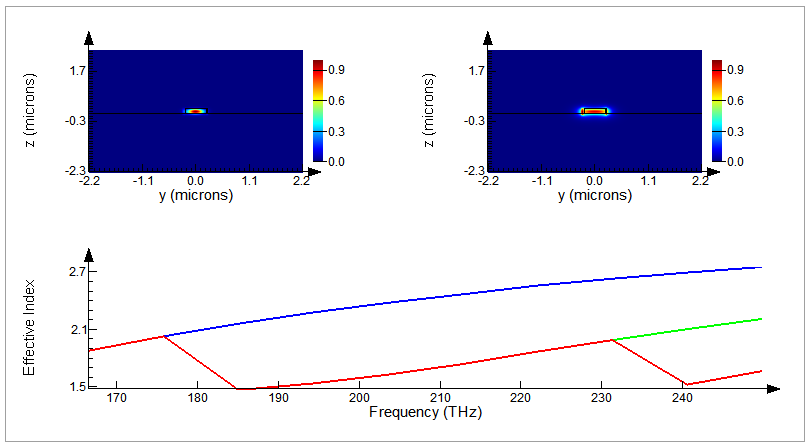
\includegraphics[width=80mm]{imagenes/FrecuencyAnalisisMode3.png}}
\caption{Simulacion de \'indice efectivo en funci\'on de la frecuencia para tres modos.
}\label{fig:FrecuencyAnalisisMode3}
\end{figure}
\begin{figure}[ht!]
\centering{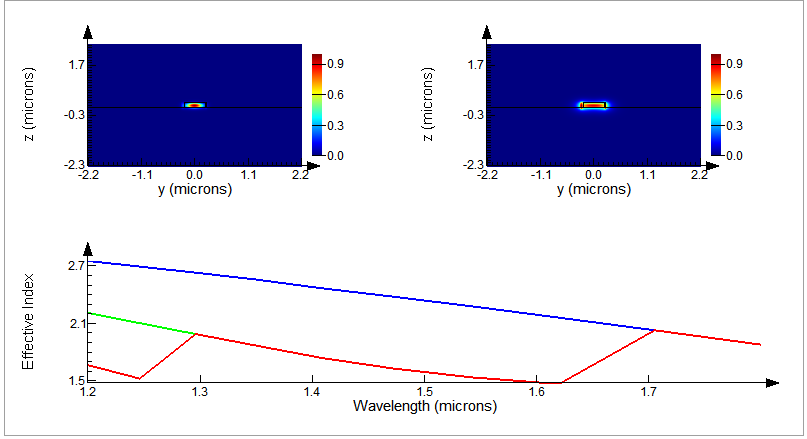
\includegraphics[width=80mm]{imagenes/Mode3Analysis.png}}
\caption{Simulaci\'on de indice efectivo en funci\'on de la longitud de onda para tres modos.
}\label{fig:Mode3Analysis}
\end{figure}
Para poder determinar la cantidad de modos que se pueden tener a medida que se var\'ia la frecuencia, partimos de las ecuaciones normalizadas  ~\eqref{eq:adimensionalEquation1}, ~\eqref{eq:adimensionalEquation2}, ~\eqref{eq:ecuacionNormalizada} y ~\eqref{eq:ecuacionNormalizada2}. Las condiciones de operaci\'on tendran cuando estas se intersecten. Si por cuestiones de simplicidad consideramos que la gu\'ia de onda es sim\'etrico, entonces las  ecuaciones normalizadas antes mencionadas se simplifican  las ecuaci\'ones ~\eqref{eq:adimensionalEquation1},~\eqref{eq:adimensionalEquation2} y resultan las dos siguientes:

\begin{equation}
\label{eq:adimensionalEquation11}
v = u\tan (u - \frac{{m\pi }}{2})
\end{equation}
\begin{equation}
\label{eq:cutoff}
\varphi  = \frac{{m\pi }}{2}
\end{equation}
Por tanto la figura~\ref{fig:ModosGuiaSimetrica} muestra la intersecci\'on entre las gr\'aficas resultantes de las ecuaciones~\eqref{eq:adimensionalEquation11} y ~\eqref{eq:frecueniaNormalizada}.
Tal y como se puede observar el radio de la circunferencia definida por la ecuaci\'on~\eqref{eq:ecuacionNormalizada} intersectado con la ordenada determina la cantidad m\'axima de modos que puede tener una gu\'ia de onda a determinada frecuencia. 
\begin{figure}[ht!]
\centering{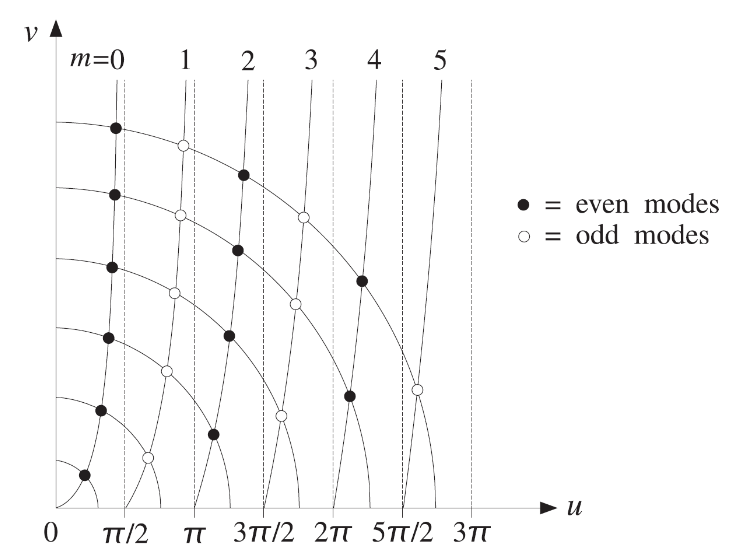
\includegraphics[width=80mm]{imagenes/ModosGuiaSLAB.png}}
\caption{Soluci\'on de los modos impares y pares de una gu\'ia sim\'etrica.Fuente:
}\label{fig:ModosGuiaSimetrica}
\end{figure}
Aplicando el mismo criterio, para el modelo asim\'etrico, a las ecuaciones~\eqref{eq:ecuacionNormalizada} y ~\eqref{eq:ecuacionNormalizada2}, se tiene que v=0 (Cruce con la ordenada), por lo tanto tenemos las siguientes ecuaciones:
\begin{equation}
\label{eq:RmSolution1}
u = {R_m}
\end{equation}
\begin{equation}
\label{eq:RmSolution2}
w = {R_m}\sqrt \delta
\end{equation}

Donde \(R_m\): Es el valor de R para el m-esimo modo m\'aximo producido en la gu\'ia de onda.
\\
Reemplazando las ecuaciones~\eqref{eq:RmSolution1} y ~\eqref{eq:RmSolution2} en ~\eqref{eq:adimensionalEquation1}, se obtiene el valor de la frecuencia para el m-esimo modo:
\begin{equation}
\label{eq:RmSolution3}
{R_m} = \frac{{m\pi }}{2} + \frac{1}{2}{\tan ^{ - 1}}(\sqrt \delta  )
\end{equation}
Si consideramos que para una frecuencia de operaci\'on cualquiera, el valor de R se encuentra fijo, entonces por la ecuaci\'on~\eqref{eq:RmSolution3} se determina la siguiente desigualdad:
\begin{equation}
\label{eq:RmInequalitySolution}
{R_m} = \frac{{m\pi }}{2} + \frac{1}{2}{\tan ^{ - 1}}(\sqrt \delta  ) \le R \Rightarrow m \le \frac{{2R - {{\tan }^{ - 1}}(\sqrt \delta  )}}{\pi }
\end{equation}
Por lo tanto el modo m\'aximo sera el valor entero m\'aximo menor o igual al valor m\'aximo de m. La cantidad m\'axima de modos es el valor del m-esimo modo aumentado en uno, teniendo en cuenta que se toma al modo cero como modo fundamental.
Con esto se concluye que a medida que se incrementa la frecuencia o se disminuye la longitud de onda la cantidad modos aumenta.
\begin{thebibliography}{}

\bibitem{1}
John, M.Senior.: `Optical Fiber Comunication Principles and Practice Third Edition',
\textit{Optical fiber waveguides}, 2009, pp. 13-61

\bibitem{2}
Katsunary Okamoto.: `Fundamentals of Optical Waveguides',
\textit{Coupled Mode Theory}, 2006, pp. 159-180

\bibitem{3}
Chin-Lin Chen: `Foundations for guided-wave optics',
\textit{Step Index thin-film waveguides, three dimensional waveguides with rectangular boundaries, optical directional couplers and their applications}, 2007, pp. 25-41, pp. 93-107, pp. 121-141

\bibitem{4}
Sophocles J. Orfanidis: `Electromagnetic
Waves and Antennas',
\textit{Waveguides, Coupled Lines},2016
\end{thebibliography}
\end{document}
